% vim:nojs:spelllang=en_us tw=76 sw=2 sts=2 fo+=awn fmr={-{,}-} et ts=8
\documentclass{beamer} % slides
%\documentclass[ignorenonframetext,handout]{beamer} % handout
%\documentclass{article}\usepackage{beamerarticle} % notes
%\usepackage[orientation=landscape,size=custom,width=16,height=9,scale=0.5]{beamerposter} 

%\includeonlyframes{curr1,curr2,curr3,curr4,curr5} % XXX

% Preamble							  {-{1

\mode<presentation>
{
  \usetheme{default} %Pittsburgh, default, boxes
  \setbeamertemplate{navigation symbols}{}
  \setbeamercovered{transparent}
  \setbeamersize
  {
    text margin left = 1.0em,
    text margin right = 1.0em
  }
  \setbeamercolor{section in toc}{fg=red}
  \setbeamercolor{section in toc shaded}{fg=structure}
  \setbeamertemplate{section in toc shaded}[default][100]
}

\usepackage[T1]{fontenc}
\usepackage[utf8]{inputenc}
\usepackage{textcomp}
\usepackage{lmodern}
\usepackage{hyperref}

\usepackage{amssymb}
\usepackage{latexsym}
\usepackage{stmaryrd}
\usepackage{extarrows}

\graphicspath{{figures/}}

\usepackage{tikz}
\usetikzlibrary{positioning,chains,matrix,shapes.arrows,scopes,
                shapes.misc,arrows,automata,calc,decorations.markings}
\everymath{\displaystyle}
\usepackage{pgf}

% Extra TikZ styles and macros {-{2

% see: 
% http://tex.stackexchange.com/questions/6135/how-to-make-beamer-overlays-with-tikz-node
\tikzset{onslide/.code args={<#1>#2}{%
  \only<#1>{\pgfkeysalso{#2}} % \pgfkeysalso doesn't change the path
}}

\tikzset{dimmedmarker/.code args={<#1> then <#2>}{%
  \alt<#1,#2>
  {
    \tikzstyle{marker} = [draw]
    \alt<#2>
    {\pgfkeysalso{->,red!80,draw opacity=.15}}
    {\pgfkeysalso{->,red!80,draw opacity=.50}}
  }
  {
    \tikzstyle{marker} = [draw=none]}
}}

\tikzset{zdimmedmarker/.code args={<#1> then <#2>}{%
  \alt<#1,#2>
  {
    \tikzstyle{marker} = [draw]
    \alt<#2>
    {\pgfkeysalso{->,blue!80,draw opacity=.15}}
    {\pgfkeysalso{->,blue!80,draw opacity=.50}}
  }
  {
    \tikzstyle{marker} = [draw=none]}
}}

\tikzstyle{every picture}+=[remember picture]
\tikzstyle{na} = [baseline=-.5ex]
\tikzstyle{ln} = [baseline,every node/.style={anchor=base,inner sep=0}]
\tikzstyle{lm} = [baseline,every node/.style={anchor=base}]

\tikzstyle{weak} =
  [decoration={markings,
               mark=at position -.6mm with {\draw[fill=white] circle (.6mm);},
               mark=at position -1.1mm with {\arrow{latex}},
              }, postaction={decorate}]

\tikzstyle{strong} =
  [decoration={markings,
               mark=at position .6mm with {\draw[fill=white] circle (.6mm);},
                  }, postaction={decorate}, -latex]

% 1 - width (e.g., .95\textwidth); 2 - image name/path
\newenvironment{hgraphicscope}[2]
  {
    \node[anchor=south west,inner sep=0] (image) at (0,0)
       {\includegraphics[width=#1]{#2}};
    \begin{scope}
    \tikzset{every node/.style={}, every path/.style={}}
    \clip (image.south west) rectangle (image.north east);
    \path let \p1=(image.south east) in (\y1, \x1) coordinate (ylimit);
    \end{scope}
    \begin{scope}[x={(image.south east)},y={(ylimit)},scale=0.1,]
  }
  {
    \end{scope}
  }

%---  }-}2------------------------------------------------------------

\newcommand{\ipause}{\onslide+<+(1)->}
\newcommand{\makepoint}[1]{\textcolor{structure}{\textbf{#1}}}

% Useful slide macros

\newcommand<>{\blue}[1]{{\color#2{blue}{#1}}}
\newcommand<>{\green}[1]{{\color#2{green}{#1}}}
\newcommand<>{\red}[1]{{\color#2{red}{#1}}}
\newcommand<>{\violet}[1]{{\color#2{violet}{#1}}}
\newcommand<>{\gray}[1]{{\color#2{gray}{#1}}}

\usepackage[final,formats]{listings}
%\lstset{language=<...>,basicstyle=\sffamily}
\input{../../../tools/lst-zelus}

%--   }-}1%%%%%%%%%%%%%%%%%%%%%%%%%%%%%%%%%%%%%%%%%%%%%%%%%%%%%%%%%%%%

\begin{document}

\begin{frame}{Backhoe example} %{-{1

\centering
\begin{tikzpicture}%{-{2
  \draw
    (0,1.25) coordinate (plant)
    +(-2.25,-1.0) [thick]rectangle +(2.25,1.0)
    +(0,-.1) node[inner sep=0] (image)
           {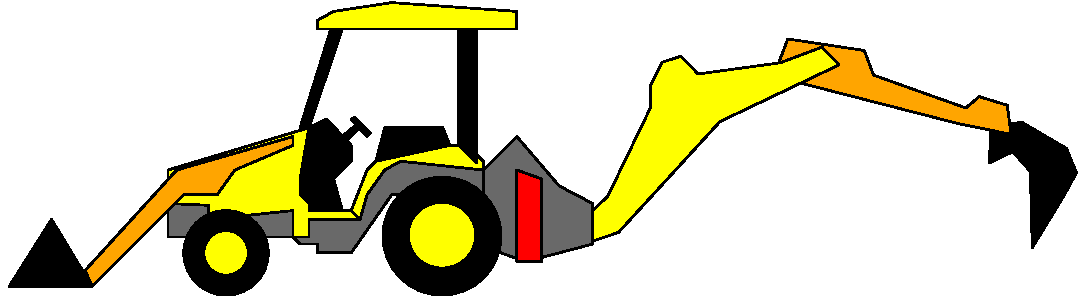
\includegraphics[width=4cm]{backhoe_loader}}
    +(-2.25,1.0) node[below right] {Plant}
    +(-2.25,0) coordinate (plantin)
    +(2.25,0) coordinate (plantout)
    ;
  \draw
    (0,-1.25) coordinate (controller)
    +(-2.25,-1.0) [thick]rectangle +(2.25,1.0)
    +(0,0) node {Controller program}
    +(2.25,0) coordinate (contrin)
    +(-2.25,0) coordinate (controut)
    ;
  \draw[very thick,->]
    (plantout) -- +(1,0) |- (contrin)
    ;
  \draw[very thick,->]
    (controut) -- +(-1,0) |- (plantin)
    ;
  \end{tikzpicture}%}-}2$

  \begin{itemize}

  \item Intended for teaching reactive programming.

  \item The \emph{controller} is a regular synchronous program.

  \item The \emph{plant} dynamics are modeled using hybrid automata and 
  first-order ODEs.

  \item The two interact via boolean flows and signals.\\
        Signals can be compared with `edge triggering'
        (\tikz{\draw (0,0) -- (.1,0) -- (.1,.25) -- (.2,.25);}%
        /\tikz{\draw (0,.25) -- (.1,.25) -- (.1,0) -- (.2,0);})
        or `function-call triggers' in Simulink.

  \end{itemize}

\end{frame}
%--   }-}1%%%%%%%%%%%%%%%%%%%%%%%%%%%%%%%%%%%%%%%%%%%%%%%%%%%%%%%%%%%%

\begin{frame}[fragile]{Modeling a segment} %{-{1

\begin{columns}[b]
\column{.4\textwidth}

\begin{lst-zelus}{\tiny}
let hybrid segment ((min, max, i), maxf, (push, pull, go))
 = ((segin, segout), angle) where

 rec der angle = v init i
 and error = v_r -. v
 and der v = (0.7 /. maxf) *. error +. 0.3 *. z init 0.0
             reset hit(v0) -> v0
 and der z = error init 0.0 reset hit(_) -> 0.0
 and v_r = if go then rate else 0.0

 and init segin = angle <= min
 and init segout = angle >= max

 and automaton
   | Stuck -> do rate = 0.0
      until push() on (angle < max) then
        do segin = false and segout = false in Pushing
      else  pull() on (angle > min) then
        do segin = false and segout = false in Pulling

   | Pushing -> local atlimit in
      do rate = maxf and atlimit = up(angle -. max)
      until atlimit on (last v > 0.3 *. maxf) then do
               emit hit = -0.8 *. last v in Pushing
      else (atlimit) then do segout = true in Stuck
      else pull() then Pulling

   | Pulling -> local atlimit in
      do rate = -. maxf and atlimit = up(min -. angle)
      until atlimit on (last v < -0.3 *. maxf) then do
               emit hit = -0.8 *. last v in Pulling
      else  (atlimit) then do segin = true in Stuck
      else  push() then Pushing
\end{lst-zelus}

\hfil
\column{.55\textwidth}

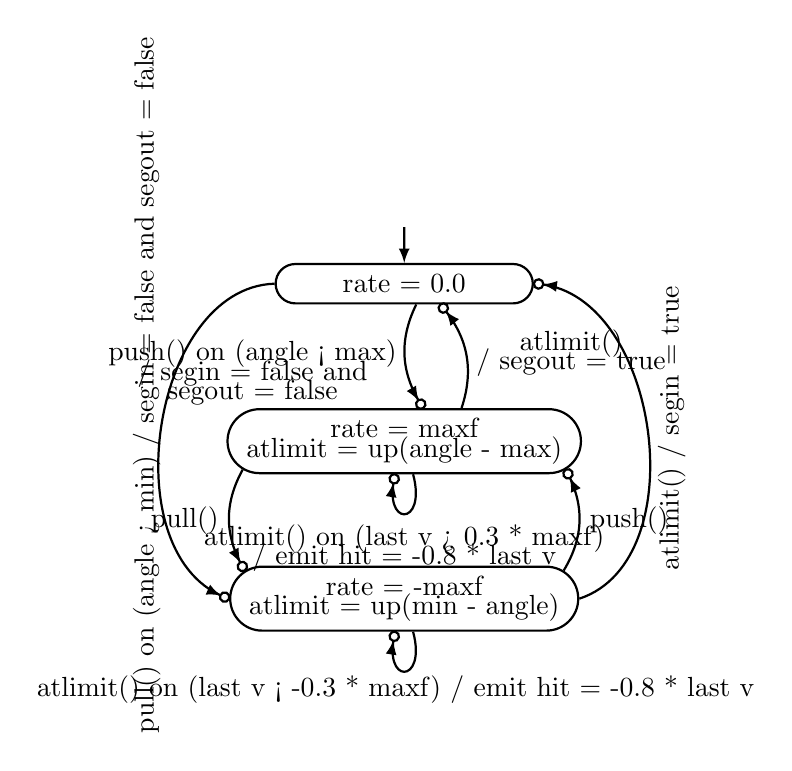
\begin{tikzpicture}[ %{-{2
    auto,
    node distance=2.0cm,
    initial text=,
    thick,
    initial where=above,
    every initial by arrow/.style={-latex},
    every loop/.style={-},
    state/.style={align=center,draw,rounded rectangle,
                  minimum width=35mm,minimum height=5mm}
  ]

  \node[state,initial] (Stuck)		 {\zlt{rate = 0.0}};
  \node[state]         (Pushing) [below of=Stuck]
    {\zlt{rate = maxf}\\[-.5em]\zlt{atlimit = up(angle - max)}};

  \node[state]		   (Pulling) [below of=Pushing]
    {\zlt{rate = -maxf}\\[-.5em]\zlt{atlimit = up(min - angle)}};

  %\node[below left=0cm and -1.5cm of Stuck]
    %{\emph{\tiny (Stuck)}};
  %\node[below left=0cm and -1.5cm of Pushing]
    %{\emph{\tiny (Pushing)}};
  %\node[below left=0cm and -1.5cm of Pulling]
    %{\emph{\tiny (Pulling)}};

  \path
      (node cs:name=Stuck,angle=300)
        edge[weak,bend right]
        node[left,pos=.65,minimum width=2.6cm,align=center]
        {\zlt{push() on (angle < max)}\\[-.5em]
          / \zlt{segin = false and}\\[-.5em]
            \zlt{segout = false}}
      (node cs:name=Pushing,angle=60)

      (Stuck.west)
        edge[weak,bend right=80]
        node[above,pos=.4,rotate=90]
        {\zlt{pull() on (angle > min)}
          / \zlt{segin = false and segout = false}}
      (Pulling.west)

      (node cs:name=Pushing,angle=190)
        edge[weak,bend right]
        node[left] {\zlt{pull()}}
      (node cs:name=Pulling,angle=170)

      (Pushing.30)
        edge[weak,bend right]
        node[right,minimum width=1.8cm,align=center]
        {\zlt{atlimit()}\\[-.5em]/ \zlt{segout = true}}
      (Stuck.-30)

      (Pushing)
        edge[weak,loop below,arrows=-]
        node[below,minimum width=5cm,align=center]
        {\zlt{atlimit() on (last v > 0.3 * maxf)}\\[-.5em]
                          / \zlt{emit hit = -0.8 * last v}}
      (Pushing)

      (node cs:name=Pulling,angle=10)
        edge[weak,bend right]
        node[right] {\zlt{push()}}
      (node cs:name=Pushing,angle=-10)

      (Pulling.east)
        edge[weak,bend right=80]
        node[below,rotate=90]
        {\zlt{atlimit()} / \zlt{segin = true}}
      (Stuck.east)

      (Pulling)
        edge[weak,loop below]
        node[pos=.70,below,align=center]
          {\zlt{atlimit() on (last v < -0.3 * maxf)}
                          / \zlt{emit hit = -0.8 * last v}}
      (Pulling)
      ;

   %\path (I) edge node {/ init} (C)
	 %(C) edge [bend left]  node {zc}    (D)
	     %edge [loop below] node {no-zc} (C)
	 %(D) edge [loop below] node {zc} (D)
	     %edge [bend left]  node {{no-zc} / reinit} (C)
	 %;
\end{tikzpicture}
\bigskip
\bigskip

\end{columns}

\end{frame}
%--   }-}1%%%%%%%%%%%%%%%%%%%%%%%%%%%%%%%%%%%%%%%%%%%%%%%%%%%%%%%%%%%%

\begin{frame}{Backhoe: sensors and actuators} %{-{1

\begin{tikzpicture}%{-{2
    []
    \tikzset{every path/.style={line width=2,dashed,color=black,
                                line cap=round},
             every node/.style={font=\ttfamily\footnotesize,
                                inner sep=1},
             title/.style={font=\bfseries\small},
             note/.style={font=\footnotesize\it}
            }
    %
    \begin{hgraphicscope}{.95\textwidth}{backhoe_loader}
        %\draw[help lines,xstep=1,ystep=1] (0,-2.5) grid (image.north east);
        \draw(0,3.2) node[title,right]
            {Sensors (plant outputs / controller inputs)}
            ;
        \draw
            (5.4,.7) -- +(0,1) node[above] {boom\_in}
            +(0,0) -- +(.5,-.5) node[right] {boom\_out}
            ;
        \draw
            (7.6,2.2) -- +(.6,.3) node[above] {stick\_in}
            +(0,0) -- +(-.15,-.7) node[below] {stick\_out}
            ;
        \draw
            (9.27,1.67) -- +(.9,-.05) node[above left=.02 and -.02] {bucket\_in}
            +(0,0) -- +(-.55,-.65) node[below] {bucket\_out}
            ;
        \draw
            (4.7,0.27) node (legsin) {} -- +(0.4,0)
            ++(0,-.27) node (legsout) {} -- +(0.4,0)
            ;
        \draw[thick,solid]
            (legsin) -- ++(-.45,-.45) -- +(-.2,0) node [left] {legs\_in}
            (legsout) -- ++(-.45,-.45) -- +(-.2,0) node [left] {legs\_out}
            ;
        \draw[thick,solid]
            (4.05,1.65) -- +(-1.5,.6)
                node[left,align=center]
                {stop\_button \\ extend\_button \\ retract\_button}
            ;
        \path[thick,solid,draw=black,fill=lightgray]
            (9.8,-0.15) circle (.3)
            node [left=.035] {second}
            +(0,0) -- +(110:.24)
            +(0,0) -- +(-30:.20)
            ;
        \draw(0,-1.1) node[title,right]
            {Actuators (plant inputs / controller outputs)}
            ;
        \path[every node/.append style={align=center}]
            (4.0,-2.0)
            +(0.0, 0.) node { legs\_extend \\ legs\_retract \\ legs\_stop }
            +(1.8,0) node { boom\_pull \\ boom\_push \\ boom\_drive }
            +(3.5,0) node (stickact)
                          { stick\_pull \\ stick\_push \\ stick\_drive }
            +(5.4,0) node { bucket\_pull \\ bucket\_push \\ bucket\_drive }
            +(-3.0,0) node { alarm\_lamp \\ done\_lamp \\ cancel\_lamp }
            ;
        \node[note,below=0 of stickact] {(pull = in; push = out)}
            ;
    \end{hgraphicscope}
\end{tikzpicture}%}-}2$

\end{frame}

%--   }-}1%%%%%%%%%%%%%%%%%%%%%%%%%%%%%%%%%%%%%%%%%%%%%%%%%%%%%%%%%%%%

\end{document}

